\section{Introduction}

\paragraph{Outline of argument:}
\begin{itemize}
\item Political discussions often revolve around underlying basic principles, especially in a polarized environment (e.g., \citealt{garrett2018moral}).
\item Moral conviction literature suggests that moralization of political attitudes should make compromise more difficult (\citealt{ryan2016no} and others).
\item However, recent studies on moral frames (grounded in MFT) show that liberals/conservatives are more likely to be persuaded when arguments are congruent with their own moral framework \citep{koleva2012tracing,kidwell2013getting}
\item Gap in the literature: few/no studies directly examined the role of moral arguments/appeals in discussions (i.e., going beyond simple framing scenarios).
\item Make a convincing argument for why \texttt{/r/ChangeMyView} is a perfect case to study the effect of moral arguments in discussions and fill this gap. Describe basic idea of the subreddit.
\end{itemize}


\section{Morality and the Potential for Compromise}

%--- Review contrasting moral foundations theory and moral conviction literature. ---

Recent years have witnessed a resurgence in partisan polarization in the United States. Politically engaged citizens hold more diverging policy
views, are more ideologically extreme, and exhibit stronger negative affect towards out-partisans than in the past \citep{hetherington2001resurgent, abramowitz2008polarization, iyengar2012affect, mason2014disrespectfully, huddy2015expressive, iyengar2015fear}. A growing literature in moral psychology---building on Moral Foundations Theory---attributes this divide (at least partially) to fundamental differences in moral frameworks that guide liberal and conservative thinking \citep[c.f.,][]{haidt2012righteous}. According to this perspective, liberals focus on \emph{individualizing} moral foundations, which include care/harm and fairness/cheating. Conservatives, on the other hand, also emphasize the remaining \emph{binding} foundations of loyalty/betrayal, authority/subversion, and sanctity/degradation \citep{haidt2007morality, graham2009liberals}. Differential emphasis on these moral dimensions is systematically related to attitudes towards a wide variety of divisive political issues \citep[e.g.][]{koleva2012tracing, kertzer2014moral, low2015moral}, personality traits like individual social dominance orientation (SDO) and right-wing authoritarianism (RWA) \citep{federico2013mapping}, as well as voting behavior \citep{franks2015using}. Overall, this body of research suggests that liberals and conservatives endorse different moral foundations and that these differences ultimately shape political attitudes, evaluations, and behavior.

An important implicit assumption in this literature is that liberals and conservatives would be more likely to come to agreements \emph{if only they focused on the same moral foundations}. For example \citet[365]{haidt2012righteous} concludes in his book \emph{The Righteous Mind: Why Good People Are Divided by Politics and Religion}: ``Once people join a political team, they get ensnared in its moral matrix. They see confirmation of their grand
narrative everywhere, and it's difficult---perhaps impossible---to convince them that they are wrong \emph{if you argue with them from outside of their matrix}'' (emphasis added). In an different article, \citet[1040]{graham2009liberals} contend that their findings ``help explain \emph{why liberals and conservatives disagree on so many moral issues} and often find it hard to understand how an ethical person could hold the beliefs of the other side: Liberals and conservatives \emph{base their moral values, judgments, and arguments on different configurations} of the five foundations.'' The underlying assumption that emphasizing the same foundations can facilitate compromise has important implications---especially in our current political environment. Somewhat surprisingly, however, it has never been subjected to a direct empirical test.

There are reasons to believe that compromise is still difficult---and potentially even further impeded---if individuals argue on the basis of the same set of moral foundations. \citet{skitka2005moral}, for example, provide a different theoretical perspective than MFT by conceptualizing moralization as a unique feature of attitude strength. According to this view, moral convictions are perceived as ``absolutes, or universal standards of truth that others should also share'' \citep[269]{skitka2010psychology}. As such, they combine the following attributes: they are viewed by individuals as applying to everyone (universality), they do not require an immediate underlying rationale but are rather seen as facts about the world (objectivity), they can be independent of authority and group norms (autonomy), they elicit strong emotional reactions, and they have an inherent motivational quality (motivation/justification) \citep{skitka2010psychology}. Building on this work, \citet{ryan2014reconsidering} argues that moral convictions are not restricted to issues that are traditionally perceived as ``moral,'' such as abortion or same-sex marriage, but can also include other issues such as economic policies. The degree of moral conviction may therefore vary between individuals as well as across issues. \citet{ryan2014reconsidering} further showed that the propensity to moralize---i.e.~the tendency to view an issue as a question of ``right and wrong''---is related to political participation, extreme political attitudes, arousal of negative emotions, and hostility. In a subsequent study, \citet{ryan2016no} suggests that moralization as a distinct characteristic of attitude intensity reorients behavior from maximizing gains to the general adherence to rules. Across multiple studies, the author shows that this tendency translates into stronger opposition to compromise about political issues and decreased support for compromising politicians. These patterns should also translate into attitudes towards---and interactions with---others who hold opposing views. Indeed, moral conviction has been shown to be related to stronger preferences for social distance from (and hostility towards) attitudinally dissimilar others and lower cooperativeness in groups holding heterogeneous views \citep{skitka2005moral}.

Ultimately, both perspectives in moral psychology lead to diverging expectations regarding the effect of moral appeals on the potential for compromise: While the moral conviction literature suggests that any type of moral appeal should make it harder to overcome disagreements, moral foundations theory contends that agreement can be facilitated if two discussants focus on the same underlying moral dimensions. Consider for example a discussion between person $\mathcal{A}$ who is set out to defend a specific opinion and person $\mathcal{B}$ who wants to challenge $\mathcal{A}$'s view and convince her otherwise. Suppose that $\mathcal{A}$ makes an opening statement justifying her opinion using moral arguments. Person $\mathcal{B}$ may then engage in the discussion and by trying to persuade $\mathcal{A}$ using either moralized or non-moralized counterarguments. Both theoretical perspectives described above suggest contrasting hypotheses regarding the persuasiveness of $\mathcal{B}$'s appeals:
\begin{center}\singlespacing\begin{tabularx}{\textwidth}{lX}
\textit{H1 (Moral Conviction)}: & Moralized counterarguments are going to be \textit{less} persuasive than non-moralized counterarguments.\\
\textit{H2 (Moral Foundations)}: & Moralized counterarguments that are congruent with the original argument's moral framework are going to be \textit{more} persuasive than non-moralized or morally incongruent counterarguments.
\end{tabularx}\end{center}

The present paper tests both competing predictions by analyzing online discussions on the Reddit community \texttt{/r/ChangeMyView}. 




\section{The Subreddit ``ChangeMyView''}
% OTHER CMV EXAMPLES:
% - Check cases 246 (discussing Haidt's theory) and 275 (on marriage equality)

Reddit is an online discussion board that is organized in thematic forums called \textit{Subreddits}. Users can join these communities based on their interests and each Subreddit has its own norms and etiquette that are enforced by voluntary moderators. \texttt{/r/ChangeMyView} (CMV) is a Reddit community where participants begin each discussion thread by stating their personal opinion on a chosen issue. Other users are invited to challenge the original poster's (OP) arguments and try to persuade them otherwise. The OP then responds to the arguments brought forward and explicitly identifies forum entries that changed his or her view by awarding a ``Delta'' ($\Delta$). The participation rules of the community foster civil exchange of arguments---even for divisive issues---and OPs are encouraged to award \(\Delta\)s genuinely.\footnote{The current set of rules for original posts as well as responses can be accessed at \url{https://www.reddit.com/r/changemyview/wiki/rules}.} To date, the Subreddit has more than 500,000 subscribed users.

As an illustrative example, consider the following discussion on marriage equality that was posted in 2014. The thread begins with the following opening statement (the posts were slightly edited to correct for spelling errors):
\begin{quote}\singlespacing
\emph{CMV: I believe that the gay marriage discussion isn't as important as the media portrays it to be.}

The real problem is the concept of marriage itself. In my view, LGBT couples are already married, regardless of the legislation that is imposed on them. Marriage isn't a set of civil rights that confirms your connection to your partner, it's the choice you make to be in private, daily, lifelong commitment to another being.

Tradition dictates that in order to be `properly' married you have to exchange vows, get a ring, and have a massive celebration (the set of traditions change based upon the culture.) but marriage isn't that, it is simple commitment to another person. The main issue that gay marriage has is that not all couples are given the same civil liberties, but this does not mean that their marriages are void. Marriage isn't decided by bystanders, it's decided by the people who live inside the union. It is for this very reason that a gay couple getting married doesn't affect your own marriage.

I've held this opinion for a while but have never had the opportunity to see if it stood up to criticism. CMV.
\end{quote}
Here, the OP argues that marriage equality should be less of a controversy since the defining feature of marriage is the commitment in a relationship rather than its legal status. Several users argued against this view from various perspectives. Below is a sample response that ultimately lead the OP to award a $\Delta$ to indicate that it changed his or her view:
\begin{quote}\singlespacing
That would be true if it was just some odd tradition. But it isn't just the ceremony, but also a tax.

Right now there is a gay tax. Gay couples have to pay higher taxes than straight couples because the government gives a tax break for married couples. The reason for this is that married couples tend to be more efficient and better for the government. The government wants to encourage marriage, so as with all things they encourage they subsidize it.

Gay people provide the exact same benefits to marriage, if not more! Adoption being the largest one.

This tax comes through in multiple ways. The yearly tax and through inheritance. The government doesn't tax inheritance as much for marriage, but if they are simply partners then they get taxed when their ``partner'' dies. 

The state also doesn't allow for gay couples see their loved ones in hospitals or prison because they aren't married.

If this was just in the church I wouldn't care. But this is much more than that.
\end{quote}
However, other discussants were less successful in persuading the OP. In contrast to the previous example, the following response did not receive a $\Delta$:
\begin{quote}\singlespacing
If gay marriage is not allowed in a state
\begin{enumerate}
\item Their marriages technically \textit{are} null and void, as the state does not recognize them.
\item Marriage is not actually decided by the people in the union, since there are legal requirements as well as legal benefits. Which brings me to my next point.
\item There are several legal benefits (as well as tax benefits) to being married. States which do not allow gay marriage do not give these legal benefits to gay couples.      
\end{enumerate}
You might believe you are married to someone, but the term ``marriage'' is a political one indeed since it has legal ramifications.
\end{quote}
While both responses emphasize the importance of legal considerations in justifying the need for marriage equality, only one of the contributions persuaded the OP sufficiently such that he awarded a $\Delta$. Ultimately, these structured online discussions on CMV provide an ideal opportunity to study the persuasiveness of moral appeals. They begin with a short explanation of a person's opinion on a given topic. Multiple users attempt to counterargue the OP's point of view from various perspectives in a civil dialogue. Most importantly, OPs explicitly identify and label arguments they found to be persuasive enough to change their views.

In a recent proceeding of the International Conference on the World Wide Web, \citet{tan2016winning} make use of this structured discussion and explore interaction dynamics on CMV by analyzing linguistic features that predict persuasiveness as well as the malleability of original posts. Their dataset includes more than 10,000 discussions that were posted on the Subreddit between January 2013 and May 2015. The analyses presented below leverage the dataset compield by \citet{tan2016winning}. In this context, it is important to note that the analysis published by \citet{tan2016winning} focuses less on the content of discussions (i.e., \textit{what is being said}) but rather examined discussion dynamics and linguistic characterics (i.e., \textit{how it is expressed}) to predict persuasiveness. The following analyses explicitly turns to the effects of moral content on discussion outcomes.

% ADVANTAGES OF CMV DATA:
% - one sided argument
% - honest labeling.

Before turning to the analysis, I want to provide a brief overview of the range of topics that are discussed on CMV. Based on the set of more than 10,000 original discussion posts included in the data, I estimated a basic topic model extracting clusters of co-occurring terms via Latent Dirichlet Allocation \citet{blei2003latent}. The topic models are based on the set of original opening statements (disregarding subsequent comments), which were pre-processed by removing numbers, punctuation, symbols, hyphens, URLs, as well as stopwords. All remaining terms were stemmed and only included if they appeared in at least 10 different posts. Figure~\ref{fig:lda} displays the average topic proportions of opening statements based on the model.

\begin{figure}[ht]
\centering
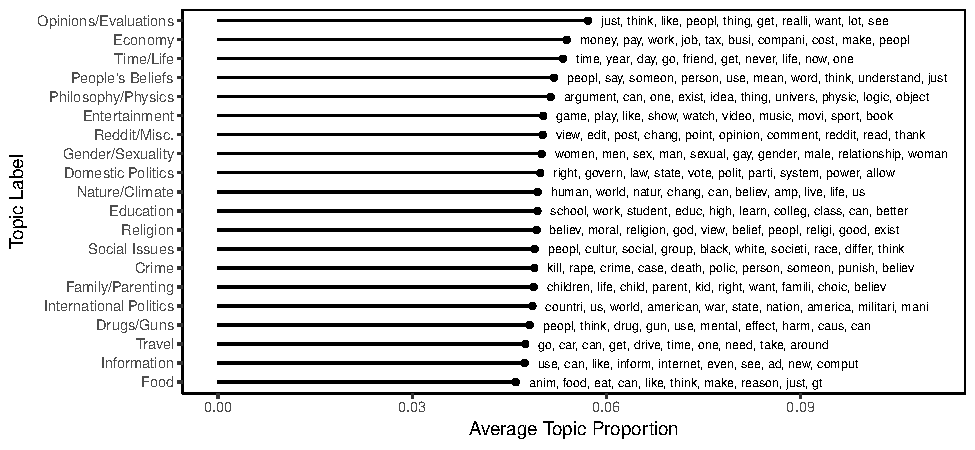
\includegraphics{/data/Dropbox/Uni/Projects/2017/cmv/calc/fig/topics.pdf}
\caption{Average topic proportions in original posts on \texttt{/r/ChangeMyView/} based on a basic LDA model with 20 topics. Figure displays the five most likely terms associated with each respective topic.}\label{fig:lda}
\end{figure}

Discussions on CMV range across a variety of topics such as economic issues, philosophy, gender/sexuality, or domestic and international politics. Additional analyses included in the appendix show that there are slight differences in the extent to which discussions on different topics ultimately result in persuasion, although these differences are surprisingly small. The following sections provide further details on the persuadability of OPs as well as the persuasiveness of specific arguments brought forward by users.


\section{Can People on the Internet be Persuaded?}


\begin{figure}[ht]
\centering
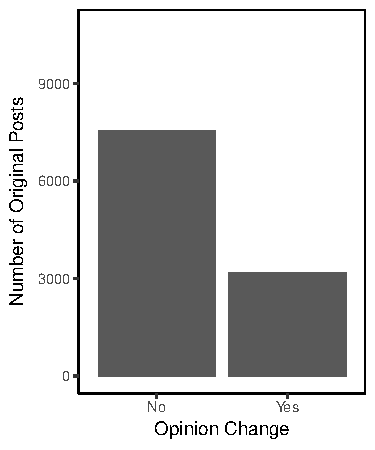
\includegraphics{/data/Dropbox/Uni/Projects/2017/cmv/calc/fig/delta.pdf}
\caption{Number of original posts on \texttt{/r/ChangeMyView/} that resulted in opinion change ($\Delta$ awarded by author) versus not.}
\end{figure}

This figure shows that OPs who use fewer moral words in their opening statements are more likely to provide a \(\Delta\) in the subsequent discussion. This basic result is consistent with the moral conviction literature.

as well as the Moral Foundations Dictionary proposed by \citet{graham2009liberals}.

\begin{figure}[ht]
\centering
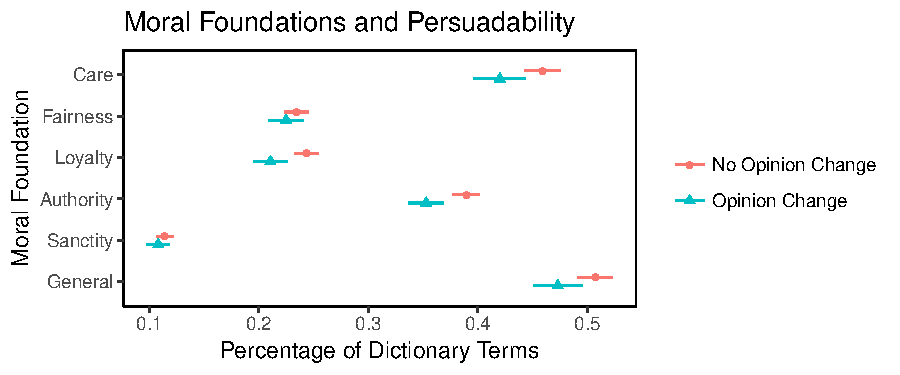
\includegraphics{/data/Dropbox/Uni/Projects/2017/cmv/calc/fig/persuadability.pdf}
\caption[Moral Foundations and Persuadability]{Moral Foundations and Persuadability: Average percentage of dictionary terms relative to the total number of words in each original post starting a discussion, comparing original posts where the author subsequently awarded a $\Delta$ (opinion change) or not (including 95\% confidence intervals).}
\end{figure}


\section{Determinants of Convincing Arguments}

\citet{tan2016winning}

The authors extract argument pairs that respond to an original post with only one being successful in changing the OPs view while being relatively similar in terms of their word choice.

{[}Elaborate on argument pair selection etc.{]}

Next, I examine the persuasiveness of moral arguments made within discussion contributions as a response to original posts that rely on any of the moral foundations.

\begin{figure}[ht]
\centering
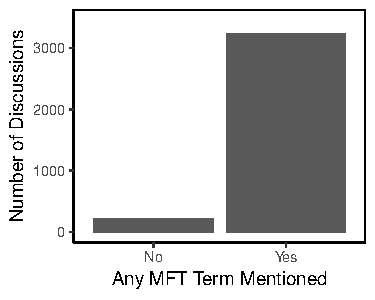
\includegraphics{/data/Dropbox/Uni/Projects/2017/cmv/calc/fig/mft_op_all.pdf}
\caption{Number of original posts in the paired argument data that included \textit{any} term mentioned in the moral foundation dictionary.}
\end{figure}


\begin{figure}[ht]
\centering
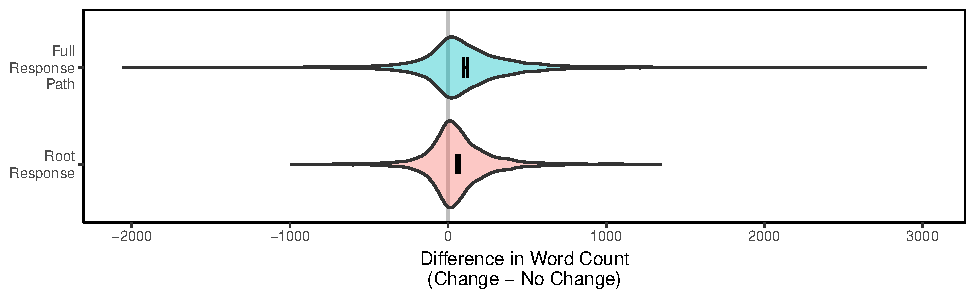
\includegraphics{/data/Dropbox/Uni/Projects/2017/cmv/calc/fig/wordcount_violin.pdf}
\caption{Something something.}
\end{figure}


\subsection{Moral Reasoning and Opinion Change}

\begin{figure}[ht]
\centering
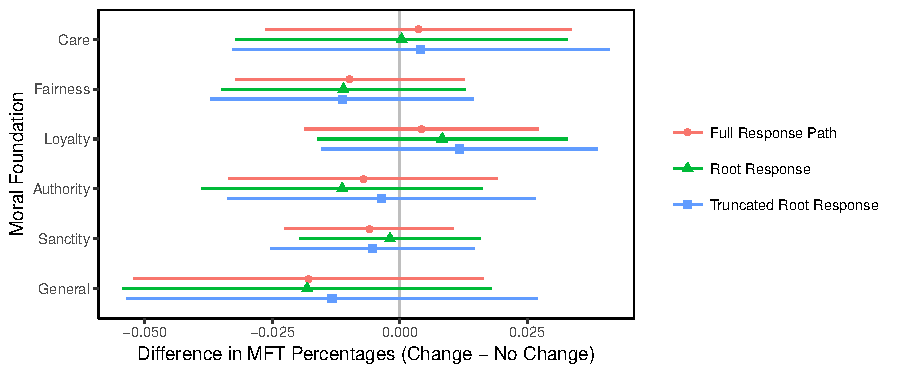
\includegraphics{/data/Dropbox/Uni/Projects/2017/cmv/calc/fig/persuasiveness.pdf}
\caption[Moral Foundations and Persuasiveness]{Moral Foundations and Persuasiveness: Average difference of dictionary term percentages relative to the total number of words in each original post starting a discussion, comparing original posts where the author subsequently awarded a $\Delta$ (opinion change) or not (including 95\% confidence intervals).}
\end{figure}


\subsection{Speaking the Same Moral Language}

Consistency in moral appeals is larger in persuasive than non-persuasive arguments.

\begin{figure}[ht]
\centering
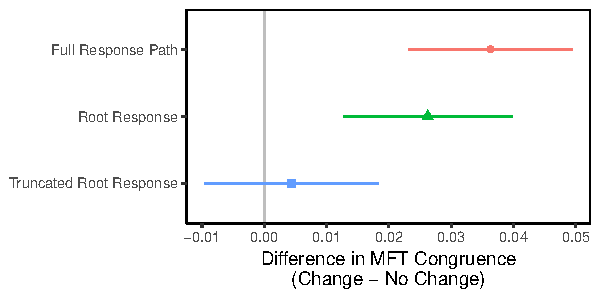
\includegraphics{/data/Dropbox/Uni/Projects/2017/cmv/calc/fig/cosine.pdf}
\caption{Yay, effects.}
\end{figure}



\section{Conclusion}\label{conclusion}

The preliminary results are consistent with moral foundations theory and contradict the previous literature on moral convictions. While the general moralization of arguments appeared to had little effects on their persuasiveness, the results show that moral congruence with initial statements are more likely to be effective in changing a person's view. As such, moral appeals can facilitate compromise and change people's minds as long as they are consistent with their existing moral frameworks. To summarize, being able to speak the same moral language might therefore help to bridge the growing divide between liberals and conservatives.

% TO DOs, future directions, etc.:
% - examine specific topics (e.g., climate change etc.)[ ]
% - clean original posts (links etc)[x]
% - adjust confidence intervals to correct for multiple comparisons [x]
% - improve code documentation, add comments in internal functions [ ]
% - check MFT scores in argument pairs (as well as OP entry) [x]
% - take into account clustering in paired data! OPs appear multiple times [ ]

% LIST for appendix:
% - distribution of response lengths
% - 
